% This .tex file (and associated .cls) produces:
%       1) The Permission Statement
%       2) The Conference (location) Info information
%       3) The Copyright Line TSConIT
%       4) NO page numbers
%       5) NO headers and/or footers
%
% Using 'sig-alternate.cls' you have control, however, from within
% the source .tex file, over both the CopyrightYear
% (defaulted to 200X) and the ACM Copyright Data
% (defaulted to X-XXXXX-XX-X/XX/XX).
% e.g.
% \crdata{0-12345-67-8/90/12} will cause 0-12345-67-8/90/12 to appear in the copyright line.
%

% This .tex source is an example which *does* use
% the .bib file (from which the .bbl file % is produced).
% REMEMBER HOWEVER: After having produced the .bbl file,
% and prior to final submission, you *NEED* to 'insert'
% your .bbl file into your source .tex file so as to provide
% ONE 'self-contained' source file.
%
% refers to the cls file being used
\documentclass{sig-alternate-br}
\usepackage{float}
\usepackage{caption}
\usepackage{subcaption}
\usepackage{hyperref}
\usepackage{xcolor}
\usepackage{enumitem}
\usepackage{tabularx}
\usepackage[numbers]{natbib}
\setlength{\bibsep}{0.0pt}
\newcommand\todo[1]{
	\textcolor{green}{#1}
}
\restylefloat{figure}
\restylefloat{table}
\begin{document}

%
% --- Author Metadata here --- DO NOT REMOVE OR CHANGE 
%\conferenceinfo{13$^{th}$ Twente Student Conference on IT}{June 23$^{st}$, 2010, Enschede, The Netherlands.}
\CopyrightYear{2015} % Allows default copyright year (200X) to be over-ridden - IF NEED BE.
%\crdata{0-12345-67-8/90/01}  % Allows default copyright data (0-89791-88-6/97/05) to be over-ridden - IF NEED BE.
% --- End of Author Metadata ---

\title{Small Data Center using Raspberry Pi 2 for Video Streaming}
% In Bachelor Referaat at University of Twente the use of a subtitle is discouraged.
 \subtitle{}


\numberofauthors{1} 
\author{ 
% You can go ahead and credit any number of authors here,
% e.g. one 'row of three' or two rows (consisting of one row of three
% and a second row of one, two or three).
%
% The command \alignauthor (no curly braces needed) should
% precede each author name, affiliation/snail-mail address and
% e-mail address. Additionally, tag each line of
% affiliation/address with \affaddr, and tag the
% e-mail address with \email.
%
% 1st. author
\alignauthor P.J.E. Velthuis\\
       \affaddr{University of Twente}\\
       \affaddr{P.O. Box 217, 7500AE Enschede}\\
       \affaddr{The Netherlands}\\
       \email{p.j.e.velthuis@student.utwente.nl}
% 2nd. author
\alignauthor 2nd Author\\
       \affaddr{2nd author's affiliation}\\
       \affaddr{1st line of address}\\
       \affaddr{2nd line of address}\\
       \email{2nd author's email address}
% 3rd. author
\alignauthor 3rd Author\\
       \affaddr{3rd author's affiliation}\\
       \affaddr{1st line of address}\\
       \affaddr{2nd line of address}\\
       \email{3rd author's email address}
}

%\additionalauthors{Additional authors: John Smith (The
%Th{\o}rv{\"a}ld Group, email: {\texttt{jsmith@affiliation.org}})
%and Julius P.~Kumquat (The Kumquat Consortium, email:
%{\texttt{jpkumquat@consortium.net}}).}
%\date{30 July 1999}


\maketitle
\begin{abstract}
This is a paper in the area of cloud computing. Cloud computing is a trend IT that customers move computing and data away from desktop and portable PCs into data centers. These data centers require a lot of power and cooling. Nowadays approximately 30\% of the data coming from these data centers is video streaming. The Raspberry Pi 2 is a low cost device that can be used in a cloud for video streaming. In this paper a further investigation in the Raspberry Pi 2 cloud is done. This research is a design research in which a design is made for a video streaming cloud consisting of Raspberry Pi's. 
\end{abstract}

\keywords{Cloud computing, Raspberry Pi 2,  micro data center, video streaming, load balancing}

\section{Introduction}
Today most of us have some data in the cloud. But despite the attention from the community, research and development of Cloud Computing services are still in its early days~\citep{tso:2013}. \newline
Cloud computing is a trend in IT that moves customers computing and data away from desktop and portable PCs into large data centers \citep{dikaiakos:2009}. In the future most internet users are expected to access internet services over lightweight portable devices requiring a lot of data bandwidth \cite{dikaiakos:2009}. This bandwidth usage causes bottlenecks. To prevent these bottlenecks people build data centers around the globe. On these data servers a lot of improvements can be made \cite{abrahamsson:2013,beloglazov:2010}. 
These data servers for example require a lot of space and cooling. There are now new technologies such as for example the powerful ARM processor. Many companies want to explore the possibilities of the Raspberry Pi 2 , because of its ARM processor and the price \cite{Pcextreme}. Some data centers already offer some cloud computing using the Raspberry Pi 2. \newline
A Raspberry Pi 2 has a power usage between the 3-5 Watt and is a small computer. A normal server has a power usage between the 75 and 250 watt~\cite{Pcextreme,beloglazov2012energy}. The low power consumption and its computing power could mean that it is better to use a Raspberry Pi 2 for specific small tasks that do not demand an entire server. For this reason research is done on the performance of the Raspberry Pi 2 in a small data center. \newline
A Raspberry Pi cloud can be the small data center for the future \cite{tso:2013}. The Raspberry is sold for 40 euro, this price makes it cheaper to do research in compared to a normal server. Building a cloud like this can be a cost effective scale model\cite{tso:2013}. It's a ideal testbed for testing distributed software. 

The Netherlands have one million subscribers for Netflix \cite{volkskrant}. Netflix is a popular video streaming service that makes HD movies watching possible. For this Netflix makes use of a content distribution network (CDN). On the internet this is known as an on demand service \cite{Adhikari:2012}. Netflix makes use of MPEG-DASH a protocol that makes streaming over HTTP possible \cite{martin:2013}. The problem is that Netflix is responsible for  29,7\% of the peak downstream traffic in US \cite{Adhikari:2012}. Because of this downstream the two main providers Comcast and  AT\&T were limiting the downstream of Netflix. This caused a lot of criticism and a new law for net neutrality has been made as a solution for this criticism \cite{net-neutrality}. \newline
In the Netherlands video streaming services such as Youtube and Netflix have an increasing amount of users. The data streaming problems coming from these increasing amount of users make it interesting to do more research in data centers with video streaming. Most of the research in computer science nowadays happen on expensive large servers \cite{tso:2013}. For this it can be very useful to see if it is possible to do research on a small computer like a Raspberry Pi 2. The problem is that we do not know if video streaming in a cloud consisting of Raspberry Pi's is possible. 

In this paper there is an investigation in how useful the Raspberry Pi 2 is in a data center with video streaming. To come to an answer the performance of the Raspberry Pi 2 is evaluated. For this the main research question is: 
\begin{center}
How well does the Raspberry Pi 2 perform in small scale data centers with video streaming? 
\end{center}

In order to come to a answer for the main question several sub-questions are researched. These sub-questions will altogether provide a answer to the main research question. 

\begin{enumerate}
	\item What are small scale data centers with video streaming and why are they used?
	\item Is the Raspberry Pi's usable for video streaming?
	\item How to fit the Raspberry Pi's into a data center considering cooling, space allocation and power?
	\item What setup does a Raspberry Pi cloud with video streaming require?
	\item How is availability in a Raspberry pi cluster with video streaming affected by various load balancing techniques? 
\end{enumerate}

This research is part literature study and a part of it is building a small Raspberry Pi cloud to analyze balancing techniques on the Raspberry Pi 2. For this research cloud video streaming is one of the specific aspects that will be investigated. The first two research questions describe the state of the art. The last three sub-questions go into the technical research that investigates the performance and possibility of Raspberry Pi's for cloud video streaming. The five sub-questions are being looked at in the next sections. Followed by a final section for conclusions and identified areas for future work.

\section{Research Methods}
This research will investigate a cloud computer consisting of Raspberry Pi's. The research method for this would be the Design Science research method. this is a method to solve field problems. This research will make use of the Design Science method proposed by Hevner~\cite{hevner:2007}. This design method has three parts. 
\begin{figure}[H]
	\centering 
	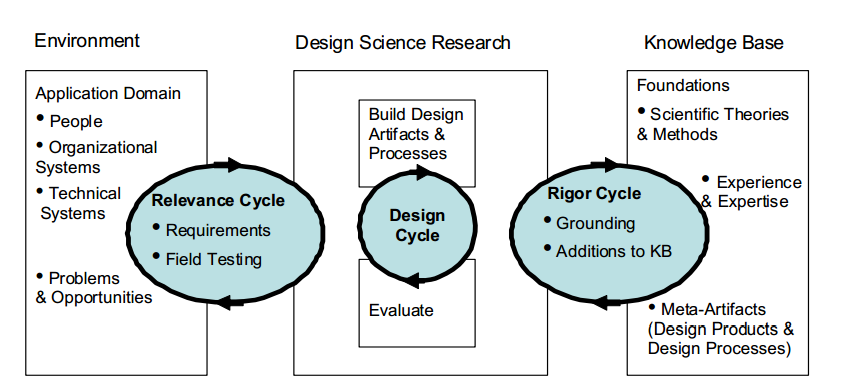
\includegraphics[width=0.4\textwidth]{Design_science.png}
	\caption{Design Science}
	\label{fig:design} %always place your label after your caption!
\end{figure}
The \textbf{relevance cycle} is important, because you first have to identify the problems and opportunities. To identify these problems we will gave some more background information in the next section. The \textbf{design cycle} is where you actually build the design. This will be highlighted in the Setup \& Experiment section. The \textbf{rigor cycle} matters because it can give you two types of additional knowledge. It provides past knowledge to ensure its invention and it's there to guarantee that the new product is a research contribution. This will for example be taken into account in the Result section. 

\todo{UML sequence diagram}

\section{Background}
\subsection{Small scale computing}
Small scale cloud computing is cloud computing with smaller computation amounts than normal \cite{cox:2014}. Most users that operate in the cloud buy the services instead of buying the hardware and having to set up the servers themselves. This service is called Infrastructure as a Service. To this specific cloud service belongs the online storage of data. The Amazon Elastic Compute Cloud (Amazon EC2) is one of the most widely used infrastructure platforms that these clients use \cite{hofer:2011}. This elasticity of computing resources is very important \cite{Miettinen:2010:EEM:1863103.1863107}. A lot of companies have their own virtual machines running in large data centers \cite{beloglazov:2010}. The advantage is that these instances can be scaled dynamically to the customer it's need. Using these instances makes easier management of the computers and varying workloads possible. 

Several cloud services have a huge demand on the network. This high demand can sometimes make it possible that data centers are unreachable.
That is a reason why many companies have their own data centers. These data centers are small and not energy efficient. Another reason why companies have their own data center is because they don't want their data to be in somebody else his hands.  Netflix a cloud service is responsible for approximately 30\% of the peak downstream traffic in US \cite{Adhikari:2012, computer-networking}. To improve this there are several data patterns possible, it can for example make a huge different in sending data in small bursts or in one large burst.

A CDN makes use of small data centers. This is because in a CDN you can get your data that is from America from a more nearby storage place. For example a website may be hosted in America. This website is connected to a CDN and in this way its possible to get your data from a more nearby server that has a copy of that website. For example if you live in Amsterdam you can perhaps get your data from London where the CDN is located instead of America. In this way the latency is decreased and there is a shorter connection distance and you have faster load times. 

Power Usage Efficiency (PUE) is nowadays becoming a more important aspect in cloud computing. Keeping the power usage low is one of the main challenges of cloud computing. The data centers now are only 12 till 20\% of the time operating, while all the servers inside are still using energy. Keeping these data centers up requires a lot of electrical power. Therefore we perhaps need to more Green Cloud Computing solutions that reduce the electrical power consumption and reduce the environmental impact of data centers~\cite{beloglazov2012energy}. For example with data centers that are using microservers. More information about this is in the next section. \newline 
With the increase of lightweight portable devices the energy efficiency becomes more important. For example can the data center do the graphic calculations needed to create a good video, however then more data needs to be send of the network. This will save energy, but will increase the data over the network. This means that a trade-off has to be made between local processing and computation offloading \cite{Miettinen:2010:EEM:1863103.1863107}. Computation offloading makes the data centers do the calculations, therefore making cloud computing more important. 

\subsection{Microserver}
Microservers come to good use in small data centers \cite{microserver}.  They are smaller in size, computer power and consume less electricity. This makes them perfect for high traffic usage tasks.  Its cheaper to a small device than a big server inside a data center, so smaller microservers make a data center more dynamic. The ability to add and remove more easily microservers can save a lot of energy. It's also better for optimization. A micro server often has a different processor compared to a normal server. ARM is a processor a micro server might use. This processor does not have so much overhead compared to a Intel one. The Intel processor is better at complex tasks, while the Arm processor is better at small tasks \cite{microserver}. The difference in these processes is because of their design. The ARM has the possibility to optimize it for a special task. In the data center of the future more of these dedicated processors will be used. 

\subsection{Streaming}\label{sec:stream}
Video streaming happens with TCP or HTTP. TCP sends frames to the client and in these frames is the video stored. Of course if the available TCP send rate is large enough then the video will play without any delays. But if the TCP send rate is less then needed then the video play will alternate between periods of continuous playout and periods of freezing~\cite{computer-networking}. Its very important that video freezing or audio playing faster then the video does not happen. This is why multimedia applications have high performance requirements. To make the video streaming possible the client will connect with video streaming service its load balancer. The load balancer will then point were which videos are stored. Here below is in a UML sequence diagram the flow displayed between the client and the video service. 
\begin{figure}[H]
	\centering 
	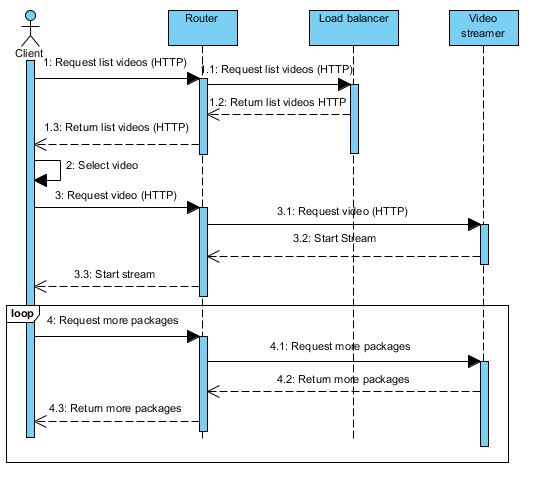
\includegraphics[width=0.4\textwidth]{VideoStreaming.jpg}
	\caption{Video stream}
	\label{fig:stream} %always place your label after your caption!
\end{figure}

As visible in the diagram you can see that there is a loop for the streaming. In this loop the client will keep requesting for more parts of the videos. Depending on the algorithm being used the amount of data requested by the client can fluctuate. For streaming a video HTTP streaming is often used. By using HTTP the client can correctly receive the video, if it receives too much data then its buffer for video playing can get full. To prevent throwing data away the server will then stop sending. To prevent throwing data away the client will have a not to large buffer. \newline
There is a important streaming technique called adaptive streaming. This streaming algorithm is often used for video on demand (VOD). It improves the experience for the end-user by adapting the video quality dynamically to the viewers network condition \cite{ffmpeg}. This techniques looks to the clients CPU possibility and it's network possibilities. It delivers small sized chunks at multiple bitrates. This techniques is used for HTTP Live Streaming (HLS). This makes use of RTMP streaming and HTTP. This way of streaming is released in 2014. It codifies video in the H.264 format.\newline
There is another special kind of HTTP streaming called DASH (Dynamic Adaptive Streaming over HTTP)~\cite{computer-networking}. In DASH the video is encoded into several different versions. If the bandwidth is high, then the client selects chunks from a high-rate version and the way around~\cite{computer-networking}. The possibility to switch between bit rate versions is in video streaming very important. To make a smooth transition between these versions possible there are intermediate versions so that the client will see less suddenly the change in video quality. In HTTP streaming the server stores the video with a different URL.   


\subsection{Video streaming and load balancing}
For video streaming several load balancing techniques can be used. There are several choices that have to be made by choosing a load balancer for a service. These choices can for example be performance, reliability and features. There can be a non-uniform demand for different movies. One solution to overcome this problem would be to replicate the most popular movies. One obvious problem is then that it is expensive in terms of storage space required. To solve this you can use dynamic replication to solve the load demand~\cite{dan1996load}. By using this you move portions of a movie to less used storage devices. The allocation of these movies only happen when there is a to high increase on one specific storage device. In this way load imbalances can be prevented \cite{dan1996load}. \newline
Load balancers are generally grouped in two layers. Layer 4 (FTP,IP, UDP, TCP )and layer 7 the application layer. Layer 7 load balancers distribute request based upon data in the application layer. Here below are some protocols and languages used for this:
\begin{enumerate}[topsep=0pt,itemsep=-1ex,partopsep=1ex,parsep=1ex]
	\item HTTP, is the hypertext transfer protocol. In section \ref{sec:stream} are mentioned some usages of this protocol. A lot of video streaming services use HTTP streaming \cite{Adhikari:2012}.  
	\item RTMP is a real time messaging protocol ~\cite{rtmp}. It is developed for streaming data between a player and a server. It is encapsulated in HTTP to traverse firewalls. It gives more video player options compared to normal HTTP thus giving the user a better experience. A disadvantage compared to normal HTTP is that it is sensitive for data spikes. These data spikes can result in a overload of the buffer which results in a empty buffer, this can lead to a stop in the video playing. 
	\item Synchronized Multimedia Integration Language (SMIL) describes multimedia presentations \cite{smil}. SMIL refers to media objects by URLs, allowing them to be shared between presentations and stored on different servers for load balancing. 
\end{enumerate}


\subsection{Video streaming in a data center}

Nowadays a lot of people watch their movies online using video streaming and this amount of people is increasing. The Netherlands have for example one million subscribers for Netflix \cite{volkskrant}. One thing that these users want is the on demand video streaming. They do not want to store the data itself and they want to have a wide choice of different videos. Netflix is a video streaming service that makes HD movies watching possible. This is known as a on demand service. For this Netflix makes use of a content distribution network (CDN). They make use of amazon its AWS, simpleDB , S3 and Cassandra for file storage \cite{Adhikari:2012}. Netflix makes use of MPEG-DASH a protocol that makes streaming over HTTP possible. To make this possible Netflix does several things in the cloud. 

 \begin{enumerate}[topsep=0pt,itemsep=-1ex,partopsep=1ex,parsep=1ex]
 	\item Content ingestion, this means that Netflix receives the studio master version of the movies and uploads these to the cloud. 
 	\item Content processing, this means that in the cloud many different formats are created for each movie.
 	\item Uploading different versions to the CDN,	this means that all the versions that have been made are distributed over the CDN.
 \end{enumerate}
Netflix ~\cite{Adhikari:2012}




\subsubsection{Video stream CDN}
Video streamer Netflix has  it's own CDN. This CDN is fully operational in 2015 and now they still use some other CDN's like Akamai. Reasons for having an own CDN is that the load balancing can be better improved. The CDN that Netflix has created is called Open Connect. To make their CDN possible they work together with the ISP providers. They use high performance HTTP delivery to get the content to the users. By having their own CDN they can get the video's faster to their users, because they can optimize their video stream algorithms for their own CDN. Besides this its possible that in this way the data going over the network can be decreased.


\section{Related work}

There have been several cloud projects with the Raspberry Pi. \newline
One of these has been the supercomputer build by Southampton~\cite{cox:2014}. Here they build it with 64 raspberry Pi's . They used a Message Passing interface to communicate between the Raspberry Pi's. The research was done in order to see what the performance of a low-power high performance cluster is. \newline
The project of the university of Glasgow~\cite{tso:2013}. This data center has 56 Raspberry Pi's. It is build for research and education purposes for a cloud data center. They have a Hadoop running on their servers. \newline
There was another project called the Beowulf cluster~\cite{beowolf-setup}. This project was created for a PhD assignment. This cluster is build for collaboratively processing sensor data.  A Beowulf cluster is simply a collection of identical, commodity computer hardware based systems~\cite{beowolf-setup}. The big advantage of the Raspberry Pi in this project was that it is cheap and it does not need a cluster administrator to watch over everything you do. 

For Video streaming there are several projects. These projects are often done by service providers such as Google with their video streamer Youtube. \newline
NGINX is busy with their Video streaming project. NGINX works together with Netflix to give users the best video watching experience. NGINX is a scalable service with high performance load balancing.  Netflix is together with NGINX busy with their project Open Connect. This project wants to improve the load balancing for video streaming over the whole network. \newline
Another service is WOWZA \cite{wowza}. WOWZA provides video streaming for a lot of companies and universities. WOWZA has done several projects for video streaming and has build with the University of Maine a content management system for their online videos. 
One mayor video stream service is of course Youtube \cite{youtube}. Youtube was once started as a project with the aim to remove the technical barriers to share videos online. Nowadays Youtube is still working hard on optimizing their video streaming service. Youtube has a online API so developers can join in and start their own projects. Youtube has its own projects for example helping mobile gamers stream their video, helping with live streaming and many more.

\section{System description}\label{sec:system}

\begin{figure}[H]
	\centering 
	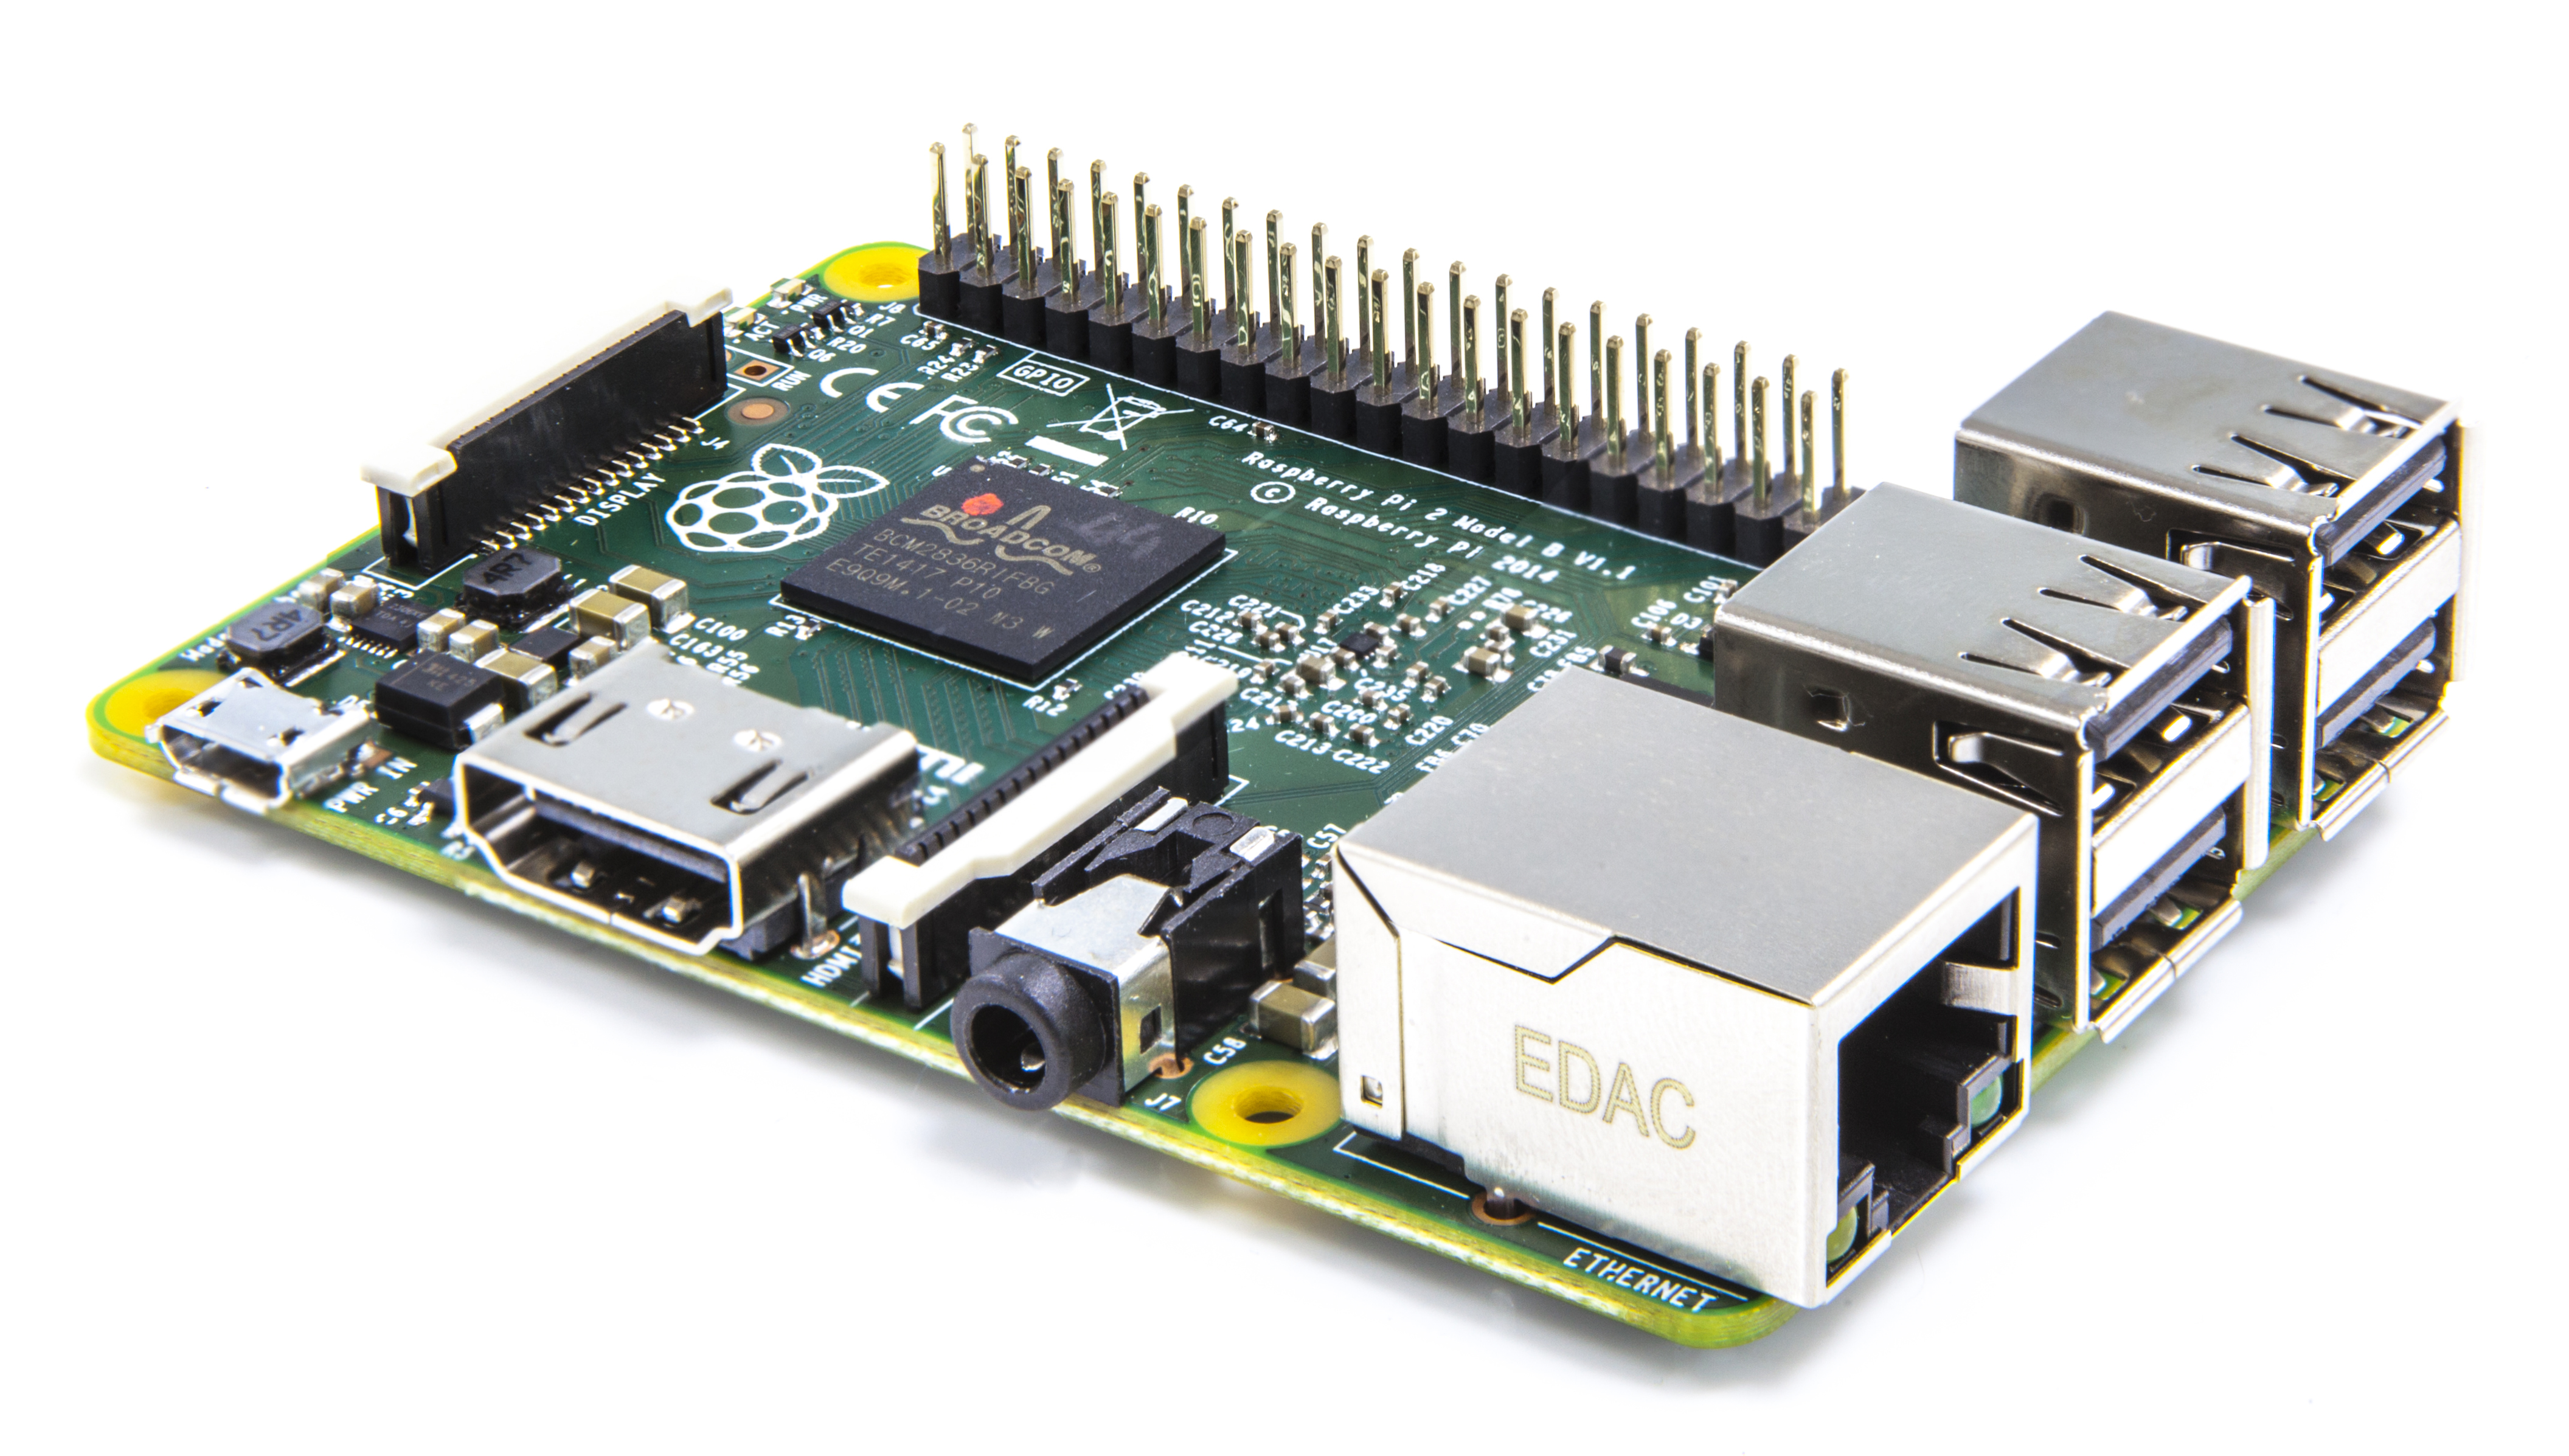
\includegraphics[width=0.4\textwidth]{Pi2ModB1GB_-comp.jpeg}
	\caption{Raspberry Pi 2 model B}
	\label{fig:raspberry} %always place your label after your caption!
\end{figure}
\begin{table}[H]
	\centering \caption{Specifications}
	\begin{tabular}{|c|c|} \hline
		Ethernet & 100 Mbps \\ \hline
		USB & 4 x USB 2.0 \\ \hline
		Video out & HDMI 1.4 \\ \hline
		Audio & 2 x analog \\ \hline
		CPU & 900MHz quad-core ARM Cortex-A7 \\ \hline
		card slot & Micro SD  \\ \hline
	\end{tabular}
	\label{tab:Specificaties}
\end{table}
The Raspberry Pi 2 (RPi 2) only consumes 3 watts, because of this it does not need active cooling. The RPi 2 does have a limited ethernet cable of only 100 Mbps. This can be a huge drawback when large amounts of data need to be distributed over the Network. It is however very useful for a investigation in load balancing for video streaming. A small network cable offers still room for analyzing the video stream. The USB 2.0 has not a huge capabilities to share the data from a external harddisk to a user, but it will be enough for this small simulation. A normal Seagate harddisks demands 10 Watt when it is actively streaming videos and when it's standby it has a consumption of 0.1  Watt.

This research makes use of three Raspberry Pi's one router and one switch. All these Pi's need power, therefore there is a power supply and 3 micro USB cables. There are three sd cards needed for the Operating System, and other software, to make the RPi 2 work. A cost structure for this can be found in the appendix section~\nameref{sec:cost}.

For some benchmark test a laptop is plugged in, so that several tests can be done from the laptop.


\section{Setup \& Experiment}


\subsection{Experiment approach}
This setup can be build by following the section \ref{sec:software} in the appendix. More details about the setup can be found in section \ref{sec:setup}. A RPi 2 is used for video streaming with load balancing. For the experiment Raspberry Pi's with a static ip address are needed. This so we can connect easily to them with SSH.  For the experiment we need a Raspberry Pi 2 that can make use of the Ethernet. This is because a RPi 2 is used as a webserver to make video streaming possible. This webserver will make video streaming possible. It will have a VPN to make it possible to put video's on the RPi 2. 
After this a cluster with one RPi 2 as a load balancer and the other two as a video stream Pi will be build. If such a cluster is made tests can be done and improvements can be made. For example some test in streaming in different quality with load balancing. The setup of the Raspberry Pi 2:

\begin{figure}[H]
	\centering 
	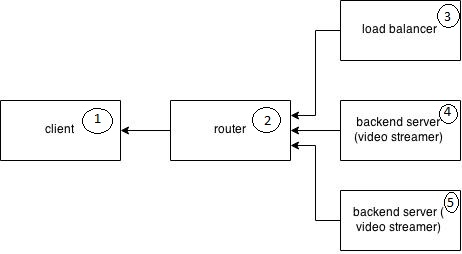
\includegraphics[width=0.5\textwidth]{raspsetup.jpg}
	\caption{Raspberry Setup}
	\label{fig:setup} %always place your label after your caption!
\end{figure}
\begin{enumerate}[topsep=0pt,itemsep=-1ex,partopsep=1ex,parsep=1ex] 
\item The client who wants to get the video. 
\item The router who redirects the client to the load balancer. The router will also have the video streamers in this network. If there are to much Raspberry Pi's in a network to connect to a single router a switch can be placed between them. 
\item The load balancer who redirects the client to the right video streamer.
\item The video streamer who streams the video to the client.
\item The video streamer who streams the video to the client.
\end{enumerate}
In the section \ref{sec:setup} the software is defined to create a cluster like this.

\subsection{Raspberry Pi 2 inside a data center}

A lot of small computers that can be turned of, instead of a few big ones that have to be on all the time can be a big step in saving energy consumed by big data centers. In this part we will look into the possibilities of doing this with the Raspberry Pi. \newline
It is possible to fit a lot of Raspberry Pi's inside a data center. PCextreme has made it possible to fit 500 Pi's inside a single data rack \cite{Pcextreme}. For this special designed boards are needed. With a special board you can for example reboot them from a distance. By having a microserver like a Raspberry Pi in a data center the hardware can be owned by only the customer, and because its in a data center there are the advantages of the high speed internet. By owning the hardware the customer will have more control over the data in the privacy and reliability aspect.\newline In this research we only have 8 Pi's and these fit easily inside the rack. The cooling of the data rack is more than sufficient to cool all these Raspberry's. The power consumption of the RPi 2 is low as you can see in table \ref{tab:cpu} below. The RPi 2 is also easy to replace inside a data center and it can easily be turned on and of, this makes it suitable inside a server rack. A problem that will exist with the Raspberry Pi 2 inside the data center is that every time a Pi's have troubles a help team inside the data center has to fix this for its customer. It is harder to get  a fully automated re-installation as for example a vServer more easily does. 

In this project a own cluster of Raspberry Pi's has been build to test its possibilities. The setup for this project looked like this:
\begin{figure}[H]
	\centering 
	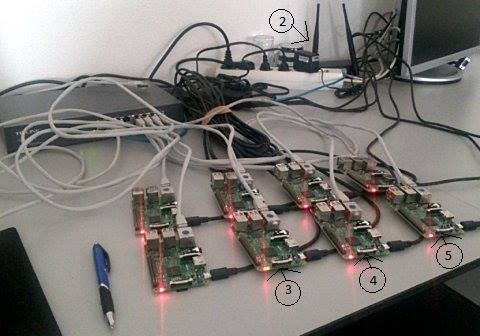
\includegraphics[width=0.50\textwidth]{setup.jpg}
	\caption{Project Setup}
	\label{fig:projectsetup} %always place your label after your caption!
\end{figure}
The figure \ref{fig:projectsetup} is photo of the project setup. This project setup is comparable with figure \ref{fig:setup}. The numbers in the front pint to the Raspberry Pi's that are also showed in figure \ref{fig:setup}. The number in the back shows the little router that is behind the power supply. In this picture there is a extra switch to connect all the Raspberry Pi's. To redo this experiment there are only three Raspberry Pi's necessary. \newline 
This setup can be placed inside of a data center. The switch and the router will then be removed and the rest will be fit nicely into the server rack. The setup that has been made now could easily fit on the project table, so that it was easy to reach them and a lot of research on them could be done. 

To verify that a Pi can operate inside a data center some tests have been done. For these tests a multimeter has been used. The Elro M990 multimeter has been used. The program sysbench has been used to run several CPU tests for the Raspberry Pi 2 its four cores. This is a benchmark test to get a quick impression about the performance of the system. The ampère and volt is measured with the multimeter during the test. the This gave the following results:
\begin{table}[H]
	\centering \caption{CPU test}
	\begin{tabular}{|c|c|c|} \hline
		Core & Ampère (A) & Volt (V)\\ \hline
		1 & 0.340 & 4.84 \\ \hline
		2 & 0.365 & 4.79 \\ \hline
		3 & 0.392 & 4.77 \\ \hline
		4 & 0.415 & 4.78 \\ \hline
	\end{tabular}
	\label{tab:cpu}
\end{table}

The idle usage of the Raspberry Pi 2 is 0.315 Ampère and 4.78 Volt. In the table there is showed that with a benchmark test of only one core the Ampère going through the system is  0.339A. There is also a read  and a memory test done which gave a voltage of 4.79 and a Ampère of 0.440-0.442.  A normal server needs about 500 watt. Each Raspberry Pi has a consumption in this test of about 2.1 watt, so about 500/2.1=238 Pi's will be possible instead of a single server. By using these small modular systems the power consumption inside a data center can be improved. The space usage however still isn't optimal, because the Raspberry Pi 2 has a micro USB cable  in one corner and an ethernet cable in the other as can be seen in figure \ref{fig:raspberry}. 
This can be solved by letting the power go over the ethernet by using a Power over Ethernet cable and a switch that is suitable for this technology. Another solution can be by making a motherboard on which you can plug in Raspberry Pi modules instead of a whole device. This is something that can be done in future work. 

\subsection{Raspberry Pi 2 setup}\label{sec:setup}
In this setup we are going to make a Netflix kind of video stream service. \newline
\textbf{Dietpi} is the software we use as operating system \cite{dietpi}. This is a diet version of Raspbian the normal Raspberry Pi operating service. The Raspbian again is a diet version of Linux. This makes that Dietpi only has the most necessary software to operate. In this way the memory usage for the operating system stays low. This low memory usage is important, because the creation of different video formats requires a lot of process power. For most systems you want as less unnecessary overhead as possible. \newline
\textbf{NGINX}~\cite{nginx}: For the load balancing and streaming over HTTP NGINX will be used. NGINX has a efficient algorithm to do HTTP load balancing. A RTMP module from Arut for NGINX will be used to make a media streaming server over HTTP \cite{arut}. This is a efficient algorithm to transfer the HTTP with RTMP encapsulated data to the users. NGINX is optimized for ARM. This is a processor the Raspberry Pi 2 is using. One other reason to choose for NGINX and not for a apache webserver is that it uses less memory. NGINX has a more efficient model than apache, and because of this it can handle more HTTP requests. Besides this is for NGINX and Apache the most documentation available on how to do video streaming. \newline
\textbf{FFmpeg} is a cross-platform solution to record, convert and stream audio and video \cite{ffmpeg}. Using this software makes adaptive streaming and streaming in different formats possible. \newline
\textbf{JW Player}~\cite{jwplayer}: JW Player is a HTML5/flash embedded media player. It is a open source media player. Besides this also JW player can make it possible to do some load balancing dependable on the bit rate that is coming from the video. It supports dynamic streaming, dynamic streaming consists of multiple single streams with the same content, all in a different quality \cite{jwplayer}. from different streams. The Player uses server modules to stream the video to the client using the formats HTTP FLV or H264.\newline
\textbf{Cassandra} is a database that helps replicating data across multiple data centers \cite{cassandra}. In the case of this project there are videos stored. This data can automatically be replicated across the nodes for fault-tolerance. In this way its possible to have the data still available when a node crashes.


\subsection{Raspberry Pi 2  testing}

In this testing section several test will be done these are: 
\begin{enumerate}[topsep=0pt,itemsep=-1ex,partopsep=1ex,parsep=1ex] 
	\item CPU test
	\item Iperf test
	\item RTMP stream test
	\item Video on demand test
	\item SMIL test
	\item Cassandra test for file location
\end{enumerate}

\subsubsection{CPU test}

The Raspberry Pi's are stress tested to make sure that they are operating correctly. For this the program stress for Linux is used to monitor its health \cite{stress}. Stress is a workload generator to test if the CPU, memory and I/O are working correctly. All three Raspberry Pi 2 have been tested using this program and they were working correctly. 

Another test is done with FFmpeg. FFmpeg needs a lot of CPU power to create new videos in different formats. To test this the top command of Linux was used \cite{top}. This measures the processor activity in real time. In this test a 230 MB 720p MPEG-4 (MP4 ) video has been converted into three different lower qualities videos, it required 200 \% of the CPU power. The output is a 120p, 240p and 480p video file. At 200 \% CPU 2 cores have to be used out of the four to produce the video, this would result in the fact that the Raspberry Pi can only process two videos into different formats at the same time. When you have streamers that have only limited data available they will not have all the different formats. These streamers need to quickly produce these videos to different formats and this can lead to difficulties.  \newline
If the videos are streamed by using NGINX they use not so much processor power. The CPU power that is needed for a single stream is about 2 \% and this barely increases when more clients are listening to it. This test is done by using web browsers and the Linux top command \cite{top}. 


\subsubsection{Iperf}

The internet speed is an important aspect in video streaming. According to Netflix you need about 5.0 Megabits per second to stream one HD movie \cite{netflix}. During the ipref test the RPi 2 has with the a maximum connection of  94.4 Mbps~\cite{ipref}. This would result in the possibility for a RPi 2 to stream about 18 videos at the same time. 

\subsubsection{RTMP stream test}

To stress test and see if the server is streaming correctly we use Apache JMeter~\cite{jmeter}. This test with Apache JMeter is used to see how many streams a Raspberry Pi 2 can handle. This test is done with a laptop and RPi 2. First a test case is created in Apache JMeter then a RTMP video stream is started and this is checked in a web page in a web browser. The reason to check it inside a web browser is because Apache JMeter can only measure HTTP files. The result of this test is that it can handle 25 users for streaming MPEG-4 (MP4 ) files over HTTP. If there are more users used the video might freeze, because there is to much latency. This becomes worse the more users there are this is a linear decrease. The RTMP stream used in this test streams the video only in 720p format. \newline Another test is by opening a media player like VLC were you can type in the RTMP stream address coming from the RPi 2. If the RTMP stream with the 230 MB video of 49 minutes is opened you can see that the video freezes some times do to buffering problems. This is because of the buffer length that is to long.  \newline
The RTMP stream is streaming about 800 kbit/s for a small 300 MB movie. Theoretically this would mean that according to the formula max users=bandwidth/bit rate stream it will result in 118 users. This is with the Raspberry Pi 2 having a 100 Mbit connection. As been seen in the test before it might already freeze at 25 users. This latency is introduced by the client which has not enough buffer time. Another problem is that FFmpeg is used as converter video to the RTMP stream, the use of a converter causes latency. \newline
If then a different stream is created with for example a audio file of 9 minutes there is no freezing with the VLC player. \newline To test it in the browser a JW player is embedded inside the web page. This browser stream can be maxed with the 118 users that are theoretically possible with the 800 kbit/s stream of the small movie. This is because the latency is not that high duo to the smaller screen used and the lower buffer length.
 

\subsubsection{Video on demand test}
For the video on demand (VOD) test a RTMP stream with FFmpeg has been created and NGINX was started to share the video. VLC was then opened on the laptop to see if there were any differences between VOD and a normal RTMP stream. The difference between VOD and RTMP is huge. With the use of video on demand the freezing was not visible. VOD is better equipped to load the stream then only RTMP. With only RTMP it's only possible to watch what is at that moment being played like normal television. RTMP does not adjust the bit stream depending on the quality you need, which is something VOD does.

\subsubsection{SMIL test}
By using the SMIL protocol you make it possible to choose your own video streaming rate for the same file, for example 120p or 480p version of a movie. You now can choose the quality by yourself. This is something that for example Youtube does. With SMIL there is the possibility to switch the quality depending on the amount of data that can get over the network. During the test with Apache JMeter by which 100 connections were simulated watching the video with the SMIL protocol used there was freezing when the users can not set their own quality. When it is done automatically this was not the case. In apache JMeter it was also possible to see some latency when testing the streams. To make this test possible videos of different qualities have been created. These video versions were created by FFmpeg and were the 720p, 480p, 240p and 120p version of the 230 MB video. 

\subsubsection{Cassandra test}
For the file location and database a Cassandra database has been made. This data server is also used by Netflix to keep track of it's files. It turned out that it was possible to run Cassandra after a lot of configuration for the Raspberry Pi was done. To see if Cassandra was running the Cassandra query language shell was  opened on each RPi 2. This was done by using the cqlsh command which is the command to start the cluster and its terminal. The output of the cqlsh command showed that it was connected to the cluster and the IP address of the RPi 2. 


\section{Result}

For this project a good setup for video streaming has been built. This result has be made possible with NGINX and several other programs. The Raspberry Pi 2 has made load balancing possible with NGINX and JW Player. In order to stream video to the user a RTMP message is encapsulated in HTTP for the web browser.  For the media player a RTMP stream is send to the user that is made by NGINX and FFmpeg.\newline
The Raspberry Pi 2 can make videos of different qualities with FFmpeg and it is perfectly capable of distributing these videos of the other Pi's.  The maximum RTMP stream output for my RPi 2 was for one around 800 kb/s. This data stream size can be different for the size and duration of the video that is being send. \newline
The video streaming with Video on Demand or adaptive streaming has a good performance. It is only limited to around 100 users. The RPi 2 has a rather limited connection, this makes video streaming with the RPi 2 still not to useful. However this experiment shows that the RPi 2 is capable of video streaming. In the future the Raspberry Pi 2 can be better than a normal server, because its more dedicated ARM processor. \newline
For the file location it is possible to set up a scalable Cassandra database. By using Cassandra it is possible to locate the files even if one node fails. This can be important when many Raspberry Pi's in a data center are being used. 
  

\section{Conclusion}
Small scale data centers are important for the data transfer over the internet. It can avoid internet bottlenecks. Besides that are the smaller cloud computers often better in executing small tasks instead of the bigger ones.  In an ideal case you want to have elasticity over the network. In this way you can increase and decrease the computation of a data center nearby the user, so that data does not have to travel so far. For video streaming you want the data as near to the user as possible in order to get him the best quality at the right speed, so that the video doesn't freeze. For video streaming the client needs to buffer a part of the movie. If the server is nearby then it's more easy to adjust the settings of these buffer. 

The Raspberry Pi 2 can be useful for video streaming. It can definitely be used for further research into video streaming algorithms. This can be algorithms such as video distribution algorithms. The Raspberry Pi 2 is a microserver and has a processor for small tasks which is video streaming. The Raspberry Pi 2 does have some drawbacks for video streaming, but is perfect for education purposes. \newline
It is possible to fit 500 Raspberry Pi's inside a single server rack. \newline
For the setup a diet version of the Raspbian operating system is used called Dietpi. Besides this it makes use of NGINX for the server with a streaming module for video. \newline
In the research several load balancing techniques were used. Cassandra is used in this research to distribute and locate the videos over different Raspberry Pi's. Adaptive streaming is used for Video on demand and normal RTMP streaming is used to setup streams. Improvements on those load balancing techniques were not possible in the scope of this research, but might be possible in future research. 
\todo{R3 \& R5 + any last words	 to do}

\section{Discussion}

 FFmpeg has a huge demand of the processor power and this can be a problem when a lot of videos have to be encoded. \newline
 The RPi 2 has a slow internet connection and this means that it streaming capacity is limited to only 18 videos at the same time. With a USB 2.0 gigabit adapter attached to a Raspberry Pi 2 this could increase in a 470 Megabit connection then it would be possible to stream about 94 videos at the same time. \newline
 Apache JMeter is a tool to test HTTP streaming. This can be used for doing web browsers streaming videos, but it would be more ideal to test only the RTMP stream. This turned out to be impossible with Apache. The next time there should be better looked at testing only the RTMP stream. 
 
\section{Future work}
New possibilities with faster USB and Ethernet cable. It is possible to create a gigabit connection over USB 2.0. This will make better video streaming possible and more users can be reached over the HTTP. Work together with streaming services such as NGINX to further develop video streaming services hosted by ARM processors. In the future it would also be possible to run a Cassandra service for the Raspberry Pi 2 this will make the file location of video's possible in a cluster. Netflix is currently looking for a specialist in  Peer-to-Peer distribution for their videos \cite{netflix}.  Peer-to-Peer distribution can be interesting with Raspberry Pi. Besides this it might be interesting to look into Peer-to-Peer distribution in general and for video streaming in specific, there can be taken a look into the technology and legal aspect of  Peer-to-Peer distribution. It might be that a Raspberry Pi 2 can fit more easily inside a data center by using PoE or by making a special motherboard and Raspberry Pi 2 modules instead of a whole device. 

\section{Acknowledgments}
This paper would not have been possible without the help of  student Nick Shot and PhD candidate Björn Postema. A special thanks to Björn Postema from the Design and Analysis of Communication Systems group of the University Twente, for his insight, good ideas and providing the necessary materials
for doing this research.

\bibliographystyle{abbrvnat}
\bibliography{sigproc}  % sigproc.bib is the name of the Bibliography in this case
% You must have a proper ".bib" file
%  and remember to run:
% latex bibtex latex latex
% to resolve all references
%
% ACM needs 'a single self-contained file'!
%
\vspace{50 mm}

%APPENDICES are optional

\clearpage
\appendix

\section{Cost structure}\label{sec:cost}
\begin{figure}[H]
	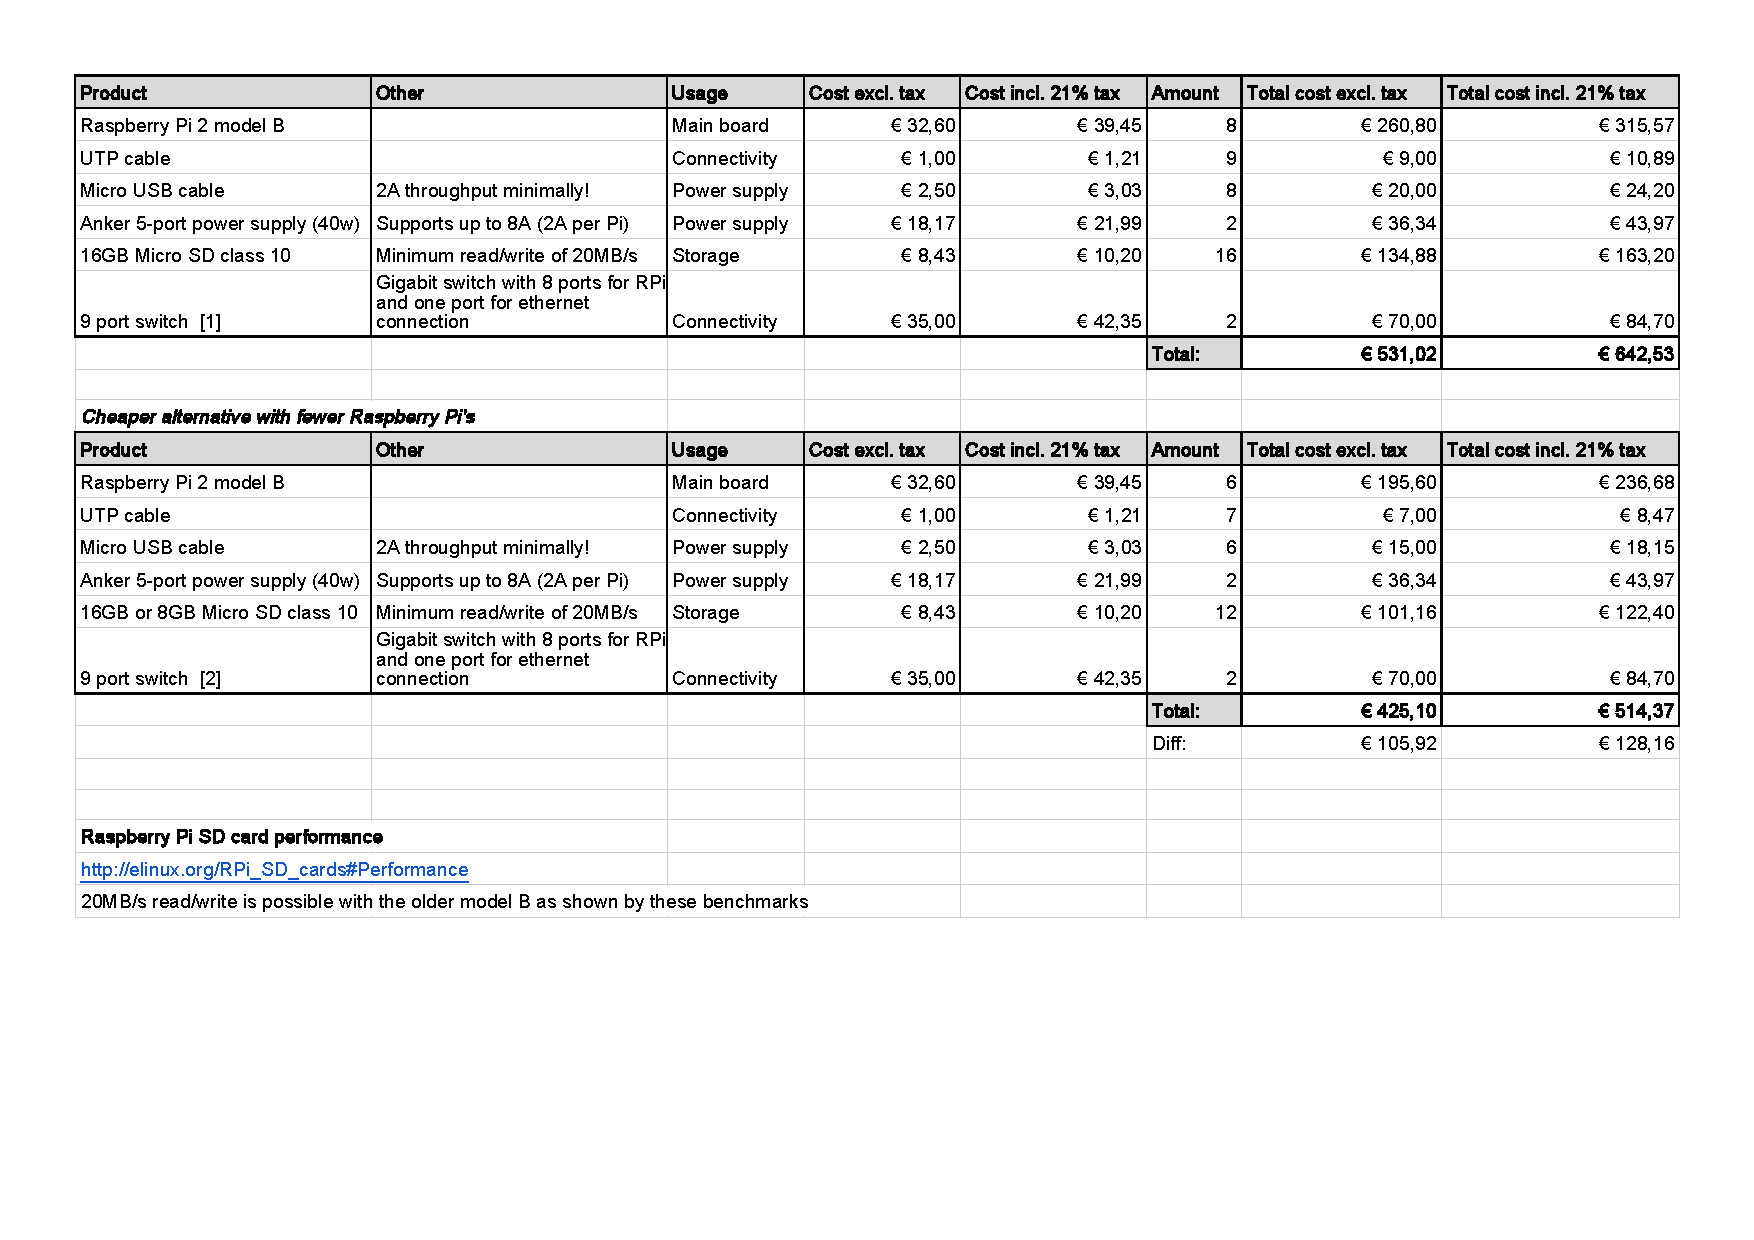
\includegraphics[scale=0.65]{Kostenoverzicht_cluster.pdf}
	\label{fig:cost}
	\caption{Cost structure}
\end{figure}


\section{Software configuration and testing}\label{sec:software}

\subsection{Raspberry Pi 2}

\subsubsection{GitHub}
For more information about the project its possible to see the GitHub repository. Comments or questions about the code can be asked in the repository. \newline
The link is: \newline
\url{https://github.com/PaulVelthuis93/bachelorreferaat}

\end{document}